\newpage

\chapter{Lezione 3: 11/03/2025}

La scorsa lezione abbiamo definito il tensore metrico:

$$
g_{ij} = \begin{pmatrix}
    g_{11} & g_{12} \\
    g_{21} & g_{22}
\end{pmatrix}
$$

Possiamo definite ora la matrice inversa $g^{ij}$ tale che il prodotto $g_{ij} \cdot g^{ij}$ sia la matrice identità.

$$
g_{ij} \cdot g^{jk} = \int_j^k (?)
$$



$$
g^{11} = \frac{g_{22}}{g}, \quad \quad g^{22} = \frac{g_{11}}{g}, \quad \quad g^{12} = g^{21} = -\frac{g_{12}}{g}
$$

dove $g$ è il determinante della matrice $g_{ij}$: $g = det g_{ij} = |\bar x_1 \times \bar x_2|$.

\vspace{1em}

Supponiamo di voler mappare lo spostamento $\Delta \Omega = \Delta u^{1} \Delta u^{2}$ di un punto $P$ da un sistema a due dimensioni ($u^1$, $u^2$) ad uno a 3 dimensioni ($x_1$, $x_2$, $x_3$) mediante la nostra trasformazione $\bar X$:



$$
\begin{cases}
\Delta x_1 = \dfrac {\partial \bar x}{\partial u^1} \Delta u^1\\
\Delta x_2 = \dfrac {\partial \bar x}{\partial u^2} \Delta u^2
\end{cases}
$$

$$
\Delta A = |\Delta x_1| \cdot |\Delta x_2| \cdot \sin \theta = 
\left | \dfrac {\partial \bar x}{\partial u^1} \Delta u^1 \right |
\left | \dfrac {\partial \bar x}{\partial u^2} \Delta u^2 \right |
\sin \theta = |\bar x_1| \Delta u^1 |\bar x_2| \Delta u^2 \sin \theta =
|\bar x_1 \times \bar x_2| \Delta u^1 \Delta u^2
$$

Dunque otteniamo:

$$
A = \iint_{\Omega} \sqrt{g} du^1 du^2$$

\subsubsection{Spazi Riemanniani e Pseudo-Riemanniani}

Gli \textbf{Spazi Riemanniani} sono spazi in cui la metrica è definita positiva:

$$
ds^2 > 0
$$

Gli \textbf{Spazi Pseudo-Riemanniani} sono spazi in cui la metrica è definita negativa:

$$
ds^2 
\left (
\begin{array}{c}
    > \\
    = \\
    <
\end{array}
\right ) 0
$$

\begin{exampleblock}[Sfera]
    La sfera è uno spazio Riemanniano:
    $$
    \begin{cases}
    ds^2 = R^2 \cos^2 v du^2 + R^2 dv^2 \\
    - \pi < u < \pi \\
    - \frac{\pi}{2} < v < \frac{\pi}{2}
    \end{cases}
    $$

    Otteniamo la matrice:

    $$
    g_{ij} = \begin{pmatrix}
        R^2 \cos^2 v & 0 \\
        0 & R^2
    \end{pmatrix}
    \quad \Rightarrow \quad
    g = R^4 \cos^2 v, \quad \sqrt{g} = R^2 \cos v
    $$

\end{exampleblock}

\begin{exampleblock}[Toro]
    Consideriamo un esmepio più complesso, il toro:

    $$
    \bar x (u, v) = [R + r \cos u] \cos v, [R + r \cos v] \sin u, r \sin v,
    $$
    
    \begin{minipage}[H]{0.5\textwidth}
        $$
        \begin{cases}
            0 < v < 2\pi \\
            0 < u < 2\pi \\
            0 < r < r
        \end{cases}
        $$
    \end{minipage}%
    \begin{minipage}[H]{0.5\textwidth}
        \begin{figure}[H]
            \centering
            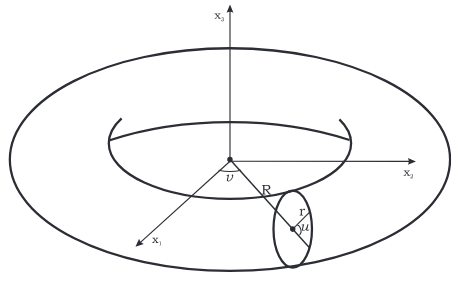
\includegraphics[width=0.6\textwidth]{assets/toro.png}
        \end{figure}
    \end{minipage}
    
    Otteniamo:

    $$
    A = \iint_{\Omega} \sqrt{g} du dv = \boxed{4 \pi^2 R r}
    $$

\end{exampleblock}

\newpage

\section{Tensori Controvarianti e Covarianti}

\subsubsection{Tensori Controvarianti}

$$
u^i = (i = 1, \dots, n) \quad \Rightarrow \quad u'^j = (j = 1, ..., n)
$$

Regola di trasformazione:

$$
du'^j = \sum_{i=1}^{n} \dfrac {\partial u'^j}{\partial u^i} du^i
$$

Otteniamo il \textbf{tensore controvariante}:

$$
\boxed{
V^{j} = \sum_{i=1}^{n} \dfrac {\partial u'^j}{\partial u^i} V^{i} 
}
$$

\subsubsection{Tensori Covarianti}

Consideriamo ora un campo scalare $\Phi$:

$$
% \begin{array}{rcl}
\partial \Phi_{'j} = \dfrac{\partial \Phi} {\partial u'^j} 
= \sum_i \dfrac{\partial \Phi} {\partial u'} \dfrac{\partial u'} {\partial u'^j}
= \sum_i \dfrac{\partial u'} {\partial u'^j} \dfrac{\partial \Phi} {\partial u'} 
= \sum_i \dfrac{\partial u'} {\partial u'^j} \partial \Phi_{'i} = W
% \end{array}
$$

Otteniamo il \textbf{tensore covariante}:

$$
\boxed{
W_{ij} = \sum_i \dfrac{\partial u'} {\partial u'^j} W_j
}
$$

$$
ds^2 = g_{ij} du^i du^j = g_{ij} \dfrac {\partial u^i}{\partial u'^l} du'^l \dfrac {\partial u^j}{\partial u'^k} du'^k = g'_{lk} du'^l du'^k 
$$

$$
g'_{lk} = \dfrac {\partial u^i}{\partial u'^l} \dfrac {\partial u^j}{\partial u'^k} g_{ij} \quad \rightarrow \quad \text{"covariante"}
$$

$$
g'^{lk} = \dfrac {\partial u'^l}{\partial u^i} \dfrac {\partial u'^k}{\partial u^j} g^{ij} \quad \rightarrow \quad \text{"controvariante"}
$$

Se un tensore ha sia indici covarianti che controvarianti, allora si dice \textbf{misto}. In tal caso è necessario applicare una trasformazione controvariante per gli indici controvarianti e una covariante per gli indici covarianti:

$$
V'^k_l = \dfrac {\partial u'^k}{\partial u^j} \dfrac {\partial u^i}{\partial u'^l} V^j_i
$$

\begin{observationblock}[Tensori e indici]
    Un tensore ha \textbf{rango} $n$ se ha $n$ indici, sia covarianti che controvarianti.

    Nota: \textit{Non tutti gli ogetti che hanno indici sono tensori}
\end{observationblock}

\newpage

Consderiamo un tensore covariante $D_i$ e un tensore metrico $g_{ij}$:

$$
D_i = g_{ij} C^j
$$


$$
D_i D^i = g_{ij} C^j D^i \quad \Rightarrow \quad 
\begin{cases}
    D_i = g_{ij} C^j\\
    C^j = D^j
\end{cases}
\quad \rightarrow \quad 
D_i = g_{ij} D^j
$$

\vspace{5em}

$$
\vec v = v^i \bar x_1
$$

$$
v_m = \vec v^i \cdot \bar x_k = v \bar x_i \bar x_k = v^i g_{ik}
$$

Consideriamo un vettore $A$:
